% ---------------------------------------------------------------------
% HEADER
% Formålet med å legge header til et eget dokument er å garantere at
% oppsettet av dokumentene er likt for alle løsningsforslagene.
% I headeren skjer følgende:
% (1) Dokumentet blir startet
% (2) Pakker blir importert
% ---------------------------------------------------------------------
% ---------------------------------------------------------------------
% HEADER
% Formålet med header er å importere de samme pakkene i alle dokumentene.
% ---------------------------------------------------------------------

% Sett opp dokumentet. Her kan 'twoside' brukes for printing
\documentclass[12pt, a4paper]{article}

% Vi trenger utf-8 for å bruke norske bokstaver: Æ, Ø, Å
\usepackage[utf8]{inputenc}

% Vi setter babel til norsk, da får dokumentegenskaper norske titler
\usepackage[norsk]{babel}

% For å kunne bruke grafikk
\usepackage{graphicx}
\newcommand{\figwidth}{0.75}

% Matematikkpakker fra AMS - American Mathematical Society
\usepackage{amsmath, amsthm, amsfonts, amssymb, mathtools}

% For eventuelle linker, e.g. \href{URL}{text}
\usepackage{hyperref}

% For headers og footers med eventuell logo
\usepackage{fancyhdr}

% Sett marginer manuelt
\usepackage[top = 3cm, left = 3cm, right = 3cm, bottom = 3cm]{geometry}

% For enkle lister, nyttig for oppgave a), b), c), ...
\usepackage[sharp]{easylist}

% Dersom flere kolonner er ønskelig i deler av dokumentet
\usepackage{multicol}

% For luft mellom paragrafer
\usepackage{parskip}

% For logikk assosiert med logoer
\usepackage{ifthen}

% For å finne totalt antall sider
\usepackage{lastpage}

% Annet
\usepackage{enumitem}

\usepackage{polynom}% Polynomer
\polyset{style=C, div=:}

\usepackage{systeme}% Likningssystemer

% Kan brukes når noe stryker ut noe, f.eks 1/n * n, her kan man ta \frac{1}{\cancel{n}} * \cancel{n}
\usepackage{cancel}



% ---------------------------------------------------------------------
% DOKUMENTVARIABLER
% ---------------------------------------------------------------------
\newcommand{\fagkode}{R1}
\newcommand{\semesteraar}{høsten 2017}
\newcommand{\forfatter}{Anita G.}
\newcommand{\dokumenttittel}{Løsningsforslag -- Eksamen \fagkode, \semesteraar}

\usepackage{siunitx}


% Set til 'true' og oppgi logo dersom du vil bruke en logo
\newboolean{bruklogo}
\setboolean{bruklogo}{false}
\newcommand{\logonavn}{}



% ---------------------------------------------------------------------
% SETUP
% Formålet med å legge setup til et eget dokument å garantere at headers,
% footers, og øverste del av dokumentet er likt for alle
% løsningsforslagene.
% ---------------------------------------------------------------------
% ---------------------------------------------------------------------
% HEADER
% Formålet med setup er at dokumentene ser rimelig like ut.
% ---------------------------------------------------------------------


% ---------------------------------------------------------------------
% Alternativ font. Kommentert ut fordi Computer Modern (default) er pen
%\usepackage{kmath,kerkis}
%\usepackage[T1]{fontenc}
% ---------------------------------------------------------------------


% ---------------------------------------------------------------------
% Sett opp headers og footers
\ifthenelse{\boolean{bruklogo}}{
% Dersom logo skal brukes, sett logoen oppe til høyre med bredde 4 cm
	\rhead{\includegraphics[width=3.5cm]{\logonavn}}
}{
% Dersom logo ikke skal brukes, sett tom header
	\rhead{}
} 
\rfoot{\thepage}
\cfoot{}
\lhead{}
\lfoot{{\scriptsize Forbedringsforslag? Bidra på \url{https://github.com/tommyod/matte_eksamener_VGS}.}}
\renewcommand{\headrulewidth}{0pt}
% ---------------------------------------------------------------------


% ---------------------------------------------------------------------
% To streker under svaret
\def\answer#1{\underline{\underline{#1}}}
% ---------------------------------------------------------------------


% ---------------------------------------------------------------------
% Start selve dokumentet
% ---------------------------------------------------------------------

\begin{document}
\pagestyle{fancy}
{\bfseries \Large \dokumenttittel} \\
{ \footnotesize Laget av \forfatter 
	\hfill Sist oppdatert: \today 
	\hfill Antall sider: \pageref*{LastPage}}
\hrule
\vspace{1em}
\begin{center}
\fbox{\fbox{\parbox{.90\textwidth}{
	Dette dokumentet er open-source;
	alle kan bidra til å gjøre det bedre.
	Dersom du finner skrivefeil, matematiske feil, eller ser at forklaringene kan være bedre: ikke nøl med å sende inn en endring. 
	Du kan finne siste versjon, og bidra, på GitHub, se:
	\url{https://github.com/tommyod/matte_eksamener_VGS}
}}}
\end{center}


% ---------------------------------------------------------------------
% DOKUMENTSTART - Skriv løsningsforslaget nedenfor
% ---------------------------------------------------------------------	


\section*{Del 1 - uten hjelpemidler}
\subsection*{Oppgave 1}
\begin{easylist}[enumerate]
	\ListProperties(Style2*=,Numbers=a,Numbers1=l,FinalMark={)})
	# Vi skal derivere $f(x) =  3x^2 -2x +1$, og gjør dette ved hjelp av regelen $f(x) = x^n \rightarrow f'(x) = nx^{n-1}$. \answer{$f'(x) = 6x-2$}.
	
	# Her ser vi at funksjonen er sammensatt av to funksjoner: $x^2$ og $e^x$. Vi bruker derfor produktregelen. $g'(x) = 2xe^x + x^2e^x = \answer{xe^x(2+x)}$.
	
	# Her får vi bruk for kjerneregelen, der vi setter $u = x^3 -1$ som kjernen. $h'(x) = \frac{1}{u} \cdot u' = \frac{1}{x^3 -1} \cdot 3x^2 = \answer{\frac{3x^2}{x^3 -1}}$.
\end{easylist}

\subsection*{Oppgave 2}
\begin{easylist}[enumerate]
	\ListProperties(Style2*=,Numbers=a,Numbers1=l,FinalMark={)})
	
	# Her må vi ta i bruk logaritmesetningene. Disse er: 
	$\ln(ab) = \ln(a) + \ln(b)$, 
	$\ln\left(a / b\right) = \ln(a) - \ln(b)$ og 
	$\ln(a^x) = x \ln(a)$.
	
	\begin{align*}
		& 2 \ln b - \ln \left(\frac{1}{b} \right) - \ln (ab^2) + \ln \left(\frac{a}{b^2}\right) \\
		& = 2 \ln b - (\ln 1 - \ln b) - (\ln a + \ln b^2) + (\ln a - \ln b^2) \\
		& = 2 \ln b - 0 + \ln b - \ln a - 2 \ln b + \ln a - 2\ln b \\
		& = - \ln b	
	\end{align*}
	
	
\end{easylist}	

\subsection*{Oppgave 3}
\begin{easylist}[enumerate]
	\ListProperties(Style2*=,Numbers=a,Numbers1=l,FinalMark={)})
	
	# $\vec{a} - 2\vec{b} = [3,1] - 2 \cdot [4,2] = [3,1] - [8,4] = \answer{[-5,-3]}$
	
	# $\vec{a} \cdot \vec{b} = [3,1] \cdot [4,2] = 3 \cdot 4 + 1 \cdot 2 = 12 + 2 = \answer{14}$.
	
	# Hvis de to vektorene $\vec{b}$ og $\vec{c}$ er parallelle, finnes det et tall $k$ slik at $\vec{b} = k \cdot \vec{c}$. 
	
	$[4,2]  = k \cdot [t+1,3]$
	
	Dette gir oss to likninger
	
	\begin{align*}
		4 & = k \cdot (t+1) \\
		2 & = 3k 
	\end{align*}
	
	Fra likning 2 ser vi at $k = \frac{2}{3}$, og dette setter vi inn i likning 1 for å finne $t$.
	
	\begin{align*}
		4 & = \frac{2}{3} \cdot (t+1) \\
		\frac{3}{2} \cdot 4 & = t+1 \\
		\frac{12}{2} -1 & = t \\
		6 - 1 & = t\\
		t & = 5
	\end{align*}
	
	De to vektorene er parallelle dersom $\answer{t = 5}$.
	
	# $|\vec{a}| = \sqrt{3^2 + 1^2} = \sqrt{10}$
	
	$|\vec{c}| = \sqrt{(t+1)^2 + 3^2}$
	
	Her kan vi enten se ut fra utrykkene hva t må være, eller vi kan regne ut t ved å sette uttrykkene lik hverandre. 
	
	Den første metoden kan vi bruke fordi vi ser at begge utrykkene under rottegnene inneholder leddet $3^2$. For at hele uttrykket da skal være likt, må også de to andre leddene være like. Altså må $(t+1)^2 = 1^2$, og dette er tilfellet når $t = 0$ eller $t=-2$. 
	
	Slike ting er ikke alltid like lett å se, men i dette tilfellet kan vi heldigvis også finne de aktuelle $t$-verdiene ved regning. De to uttrykkene under rotegnene må fremdeles være like, og dermed får vi likningen
	
	\begin{align*}
		(t+1)^2 + 3^2 &= 10 \\
		t^2 + 2t + 1 +9 - 10 & = 0 \\
		t^2 + 2t & = 0 \\
		t(t+2) & = 0 \\
	\end{align*}
	
	Denne likningen er oppfylt dersom \answer{$t = 0$ eller $t = -2$}.
\end{easylist}	


\subsection*{Oppgave 4}
\begin{easylist}[enumerate]
	\ListProperties(Style2*=,Numbers=a,Numbers1=l,FinalMark={)})
	
	# Arealet av en trekant er gitt ved formelen $A = \frac{\textnormal{grunnlinje} \cdot \textnormal{høyde}}{2}$. I vår trekant ser vi at grunnlinjen er $g = x$ og høyden er $h = f(x)$. Da blir arealet av trekanten
	
	\begin{align*}
		F(x) & = \frac{x \cdot f(x)}{2} \\
		& = \frac{x \cdot 2(x-3)^2}{2} \\
		& = x(x-3)^2 \\
		& = x(x^2 - 6x + 9) \\
		& = x^3 - 6x^2 +9x
	\end{align*}
	
	# For å finne den $x$-verdien som gir størst areal må vi derivere funksjonen for arealet og finne toppunktet til denne. 
	
	$F'(x) = 3x^2 - 12x + 9$
	
	Vi faktoriserer den deriverte ved hjelp av nullpunktene. Disse kan finnes ved hjelp av abc-formelen. $\rightarrow F'(x) = 3(x-1)(x-3)$
	
	Deretter tegner vi fortegnslinje. Her er det lurt å være obs på definisjonsmengden til funksjonen ($0<x<3$).
	
		\begin{figure}[ht!]
			\centering
			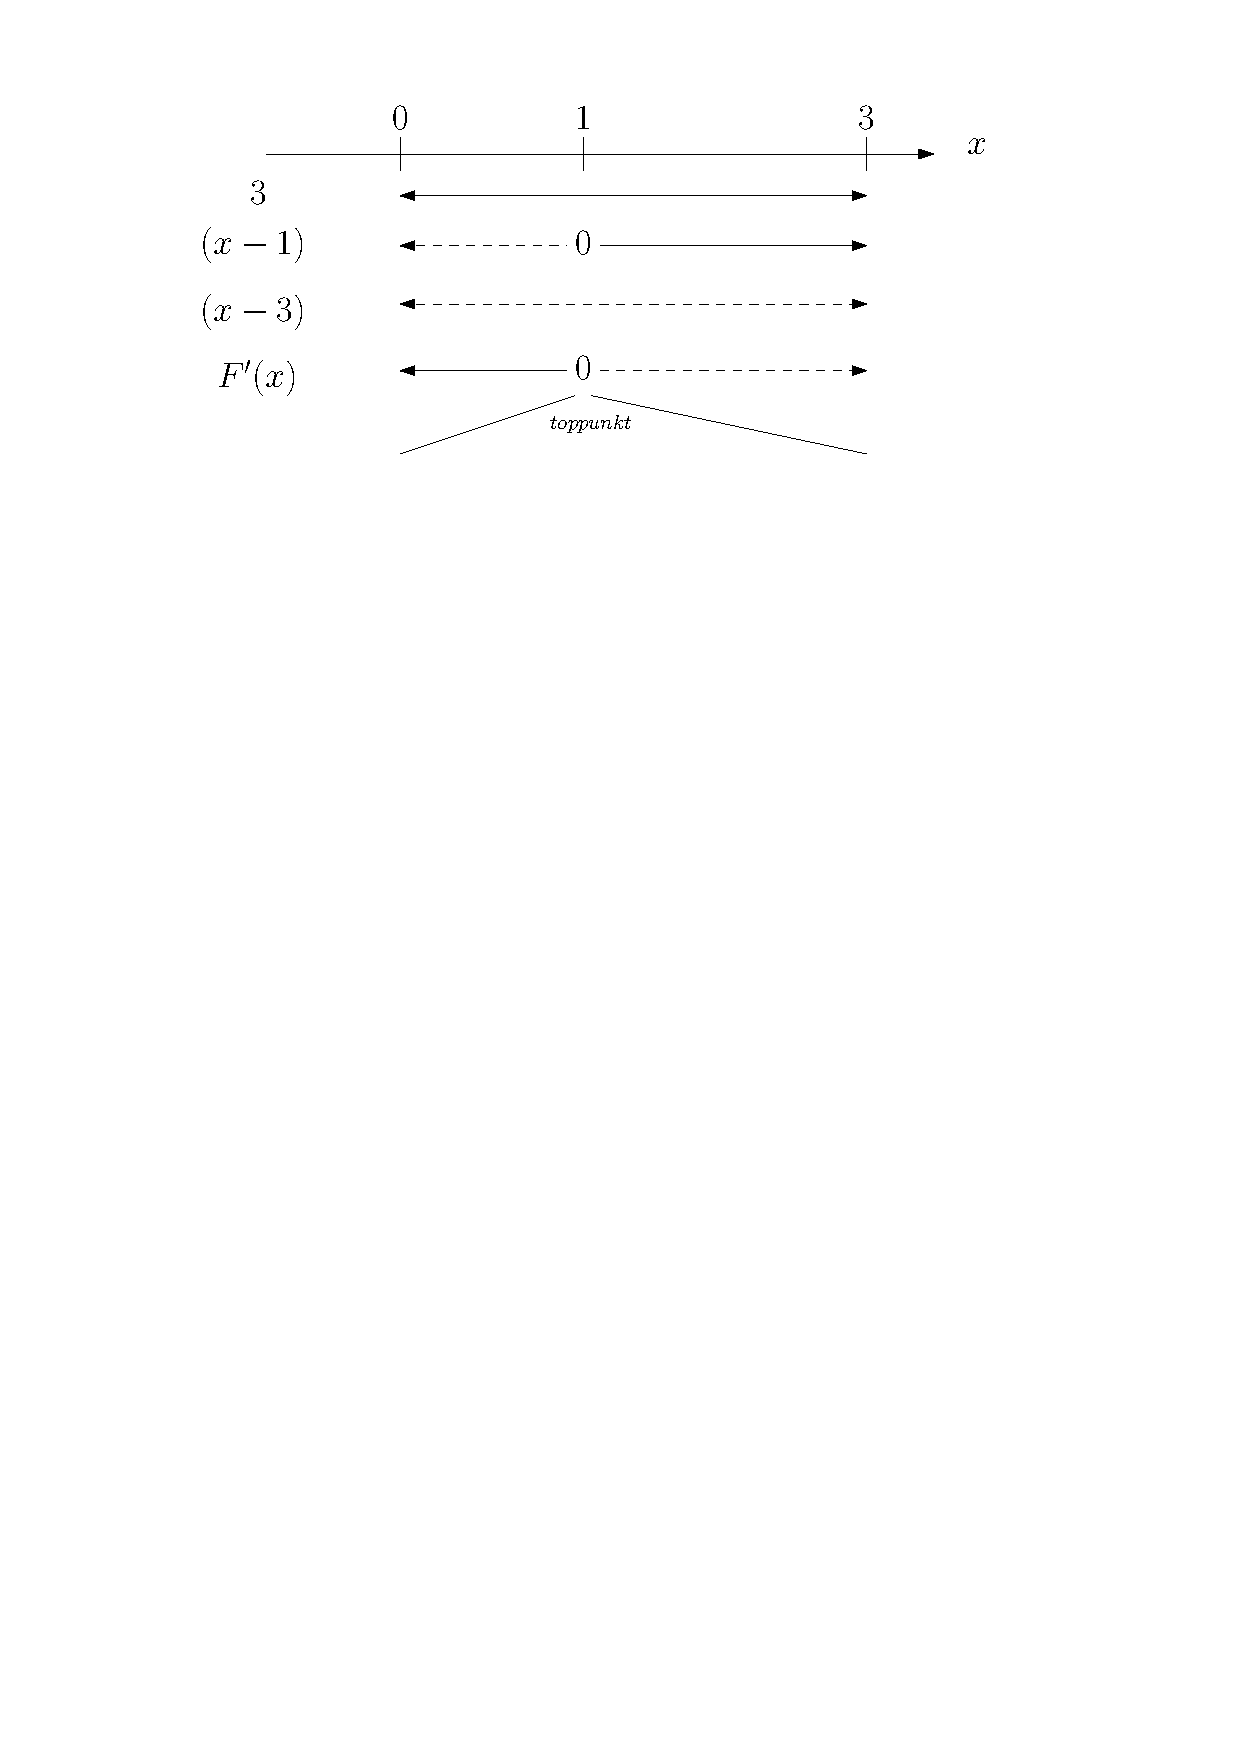
\includegraphics[width=0.725\linewidth]{figs/del1_oppg4b.pdf}
			\label{fig:del1_oppg4c}
		\end{figure}
		
		Ut i fra definisjonsmengden ser vi at det er kun $x = 1$ som gir mulighet for et toppunkt, og ut i fra fortegnslinjen ser vi at dette punktet faktisk er et toppunkt. Det vil si at \answer{arealet er størst når $x = 1$}.
	
	
	
\end{easylist}	
\end{document}